\subsection{Теорема о дифференцируемости интеграла с переменным верхним пределом. Существование первообразной у непрерывной функции, формула Ньютона — Лейбница}

Рассмотрим функцию $f(t)$, интегрируемую на отрезке $[a, b]$. Интеграл с переменным верхним пределом определяется как функция:
\[ \Phi(x) = \int\limits_a^x f(t) dt, \quad x \in [a, b] \]
Лектор отмечает, что это фундаментальный объект, связывающий интегральное исчисление с дифференциальным.

\subsubsection*{1. Теорема о производной интеграла по верхнему пределу}

\begin{theorem}
Если функция $f(t)$ интегрируема на отрезке $[a, b]$ и непрерывна в некоторой точке $x \in [a, b]$, то функция $\Phi(x)$ дифференцируема в этой точке, причем:
\[ \Phi'(x) = f(x) \]
\end{theorem}

\begin{tcolorbox}[title=Доказательство, breakable]
Для доказательства дифференцируемости найдем предел разностного отношения при $\Delta x \to 0$.

1. Рассмотрим приращение функции $\Phi$ в точке $x$:
\[ \Delta \Phi = \Phi(x + \Delta x) - \Phi(x) = \int\limits_a^{x + \Delta x} f(t) dt - \int\limits_a^x f(t) dt = \int\limits_x^{x + \Delta x} f(t) dt \]

2. Поскольку функция $f(t)$ непрерывна в точке $x$, воспользуемся теоремой о среднем для интеграла. Для достаточно малых $\Delta x$ функция $f(t)$ будет интегрируема на малом отрезке с концами $x$ и $x + \Delta x$. Тогда существует точка $\xi$, лежащая между $x$ и $x + \Delta x$, такая что:
\[ \int\limits_x^{x + \Delta x} f(t) dt = f(\xi) \cdot \Delta x \]

3. Составим разностное отношение:
\[ \frac{\Delta \Phi}{\Delta x} = \frac{f(\xi) \Delta x}{\Delta x} = f(\xi) \]

4. Устремим $\Delta x \to 0$. При этом точка $\xi$, «зажатая» между $x$ и $x + \Delta x$, также стремится к $x$ ($\xi \to x$). В силу непрерывности функции $f$ в точке $x$:
\[ \lim_{\Delta x \to 0} f(\xi) = f(x) \]

5. Таким образом, предел разностного отношения существует и равен $f(x)$, что по определению означает:
\[ \Phi'(x) = f(x) \]
\end{tcolorbox}

\subsubsection*{2. Существование первообразной у непрерывной функции}

Эта теорема дает ответ на один из важнейших вопросов анализа: для каких функций гарантированно существует первообразная.

\begin{consequence}
Любая непрерывная на промежутке функция $f(x)$ имеет на этом промежутке первообразную. Одной из таких первообразных является интеграл с переменным верхним пределом $\Phi(x) = \int_a^x f(t) dt$.
\end{consequence}

Лектор подчеркивает, что до этого момента мы умели находить первообразные только для узкого круга функций (используя таблицу производных в обратную сторону), теперь же мы имеем теоретическую гарантию их существования для всех непрерывных функций.

\subsubsection*{3. Формула Ньютона — Лейбница}

Данная формула является основным инструментом вычисления определенных интегралов через первообразные.

\begin{theorem}[Ньютона — Лейбница]
Если функция $f(x)$ непрерывна на отрезке $[a, b]$ и $F(x)$ — любая её первообразная на этом отрезке, то справедлива формула:
\[ \int\limits_a^b f(x) dx = F(b) - F(a) \]
\end{theorem}

\begin{tcolorbox}[title=Доказательство, breakable]
1. Пусть $f(x)$ непрерывна на $[a, b]$. Тогда по доказанному выше функция $\Phi(x) = \int_a^x f(t) dt$ является одной из первообразных функции $f(x)$.

2. Пусть $F(x)$ — любая другая первообразная $f(x)$ на $[a, b]$. По свойству первообразных, любые две первообразные одной и той же функции на промежутке отличаются на константу $C$:
\[ F(x) = \Phi(x) + C = \int\limits_a^x f(t) dt + C \]

3. Найдем значение константы $C$, подставив $x = a$:
\[ F(a) = \int\limits_a^a f(t) dt + C \]
Так как интеграл по вырожденному отрезку $\int_a^a f(t) dt = 0$, получаем $C = F(a)$.

4. Теперь подставим полученное значение $C$ в равенство из пункта 2 и положим $x = b$:
\[ F(b) = \int\limits_a^b f(t) dt + F(a) \]

5. Отсюда окончательно получаем формулу Ньютона — Лейбница:
\[ \int\limits_a^b f(t) dt = F(b) - F(a) \]
\end{tcolorbox}

\textbf{Геометрический смысл:}
Формула Ньютона — Лейбница связывает площадь криволинейной трапеции (определенный интеграл) с изменением (приращением) её первообразной. Если интерпретировать $f(t)$ как скорость, то интеграл — это пройденный путь, который равен разности координат $F(b) - F(a)$ в конечный и начальный моменты времени.

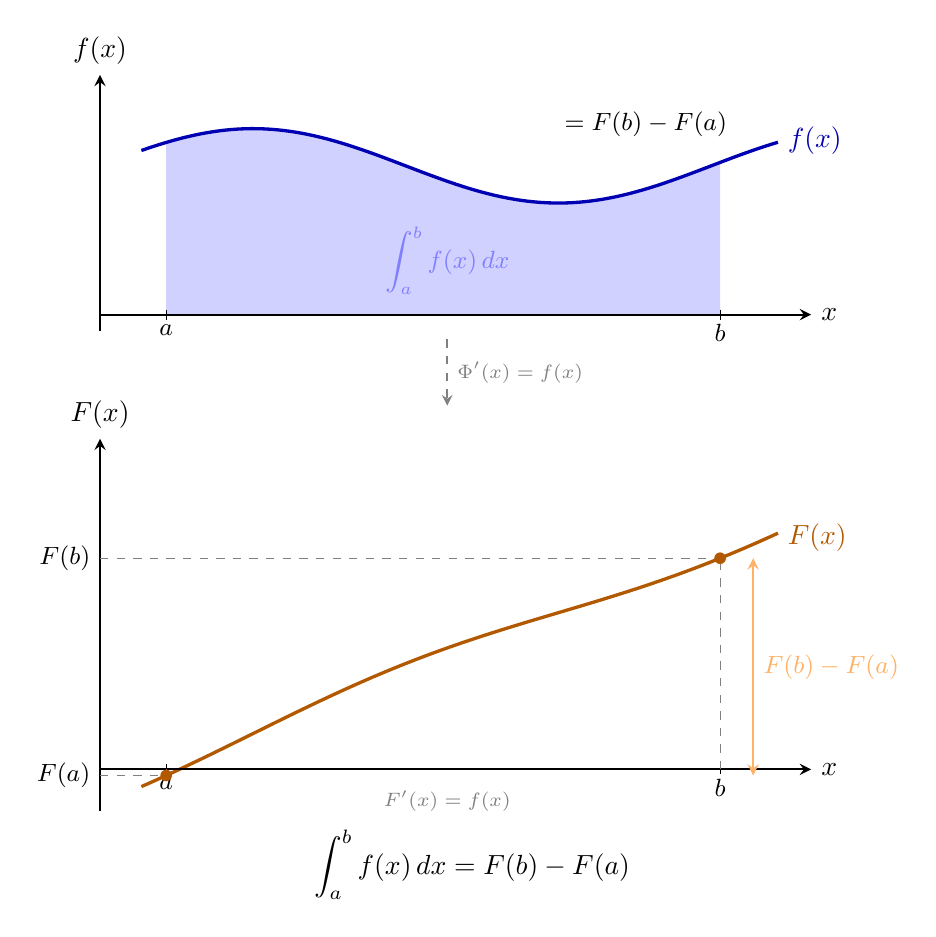
\begin{tikzpicture}[>=stealth, scale=1.05]
 
% ИСПРАВЛЕНО: #1 вместо \x в обеих функциях
\pgfmathdeclarefunction{ff}{1}{%
  \pgfmathparse{0.45*sin(deg(#1*0.85))+1.8}%
}
\pgfmathdeclarefunction{FF}{1}{%
  \pgfmathparse{-0.45/0.85*cos(deg(#1*0.85))+1.8*#1}%
}
 
\def\xa{0.8}
\def\xb{7.5}
\pgfmathsetmacro{\FaRaw}{FF(\xa)}
\pgfmathsetmacro{\FbRaw}{FF(\xb)}
% масштаб первообразной для удобного отображения
\pgfmathsetmacro{\FaS}{\FaRaw*0.22-0.3}
\pgfmathsetmacro{\FbS}{\FbRaw*0.22-0.3}
 
%=== Верхняя панель: f(x) с площадью ===
\begin{scope}[yshift=5.5cm]
  \fill[blue!18,domain=\xa:\xb,samples=80]
    plot(\x,{ff(\x)}) -- (\xb,0) -- (\xa,0) -- cycle;
  \draw[blue!70!black,very thick,domain=0.5:8.2,samples=100]
    plot(\x,{ff(\x)});
 
  \draw[->,thick] (0,0)--(8.6,0) node[right]{$x$};
  \draw[->,thick] (0,-0.2)--(0,2.9) node[above]{$f(x)$};
 
  \foreach \xp/\lab in {\xa/{$a$},\xb/{$b$}}{
    \draw (\xp,0.06)--(\xp,-0.06);
    \node[below,font=\small] at (\xp,0){\lab};
  }
  \node[blue!70!black,font=\itshape,right] at (8.2,2.1){$f(x)$};
  \node[blue!50,font=\small] at (4.2,0.65)
    {$\displaystyle\int_a^b f(x)\,dx$};
 
  % связь с F(b)-F(a)
  \node[right,font=\small] at (5.5,2.3){$=F(b)-F(a)$};
\end{scope}
 
%=== Стрелка между панелями ===
\draw[->,gray,dashed,line width=0.7pt]
  (4.2,5.2)--(4.2,4.4)
  node[midway,right,font=\scriptsize,gray]{$\Phi'(x)=f(x)$};
 
%=== Нижняя панель: F(x) ===
\begin{scope}[yshift=0cm]
  \draw[orange!70!black,very thick,domain=0.5:8.2,samples=100]
    plot(\x,{FF(\x)*0.22-0.3});
 
  \draw[->,thick] (0,0)--(8.6,0) node[right]{$x$};
  \draw[->,thick] (0,-0.5)--(0,4.0) node[above]{$F(x)$};
 
  \foreach \xp/\lab in {\xa/{$a$},\xb/{$b$}}{
    \draw (\xp,0.06)--(\xp,-0.06);
    \node[below,font=\small] at (\xp,0){\lab};
  }
 
  % пунктиры и точки
  \draw[dashed,gray,thin] (0,\FaS)--(\xa,\FaS);
  \draw[dashed,gray,thin] (0,\FbS)--(\xb,\FbS);
  \draw[dashed,gray,thin] (\xa,0)--(\xa,\FaS);
  \draw[dashed,gray,thin] (\xb,0)--(\xb,\FbS);
  \fill[orange!70!black] (\xa,\FaS) circle(2pt);
  \fill[orange!70!black] (\xb,\FbS) circle(2pt);
 
  \node[left,font=\small] at (0,\FaS){$F(a)$};
  \node[left,font=\small] at (0,\FbS){$F(b)$};
 
  % скобка F(b)-F(a)
  \draw[<->,orange!60,line width=0.8pt]
    (\xb+0.4,\FaS)--(\xb+0.4,\FbS)
    node[midway,right,font=\small]{$F(b)-F(a)$};
 
  \node[orange!70!black,font=\itshape,right] at (8.2,2.8){$F(x)$};
  \node[gray,font=\scriptsize] at (4.2,-0.38){$F'(x)=f(x)$};
\end{scope}
 
%--- Итоговая формула ---
\node[font=\normalsize] at (4.5,-1.15)
  {$\displaystyle\int_a^b f(x)\,dx = F(b) - F(a)$};
 
\end{tikzpicture}